\documentclass{article}
\usepackage{multicol}
\usepackage{xcolor}
\usepackage{graphicx}
\linespread{1.35}
\usepackage{amsmath}
\usepackage{color}
\usepackage{tikz}
\usetikzlibrary{arrows,automata}

\begin{document}


\begin{flushright}
\texttt{Finite State Machine} \hspace*{0.1cm}\textbf{$|$} \hspace*{0.1cm} \textbf{205}\hspace*{0.1cm}
\end{flushright}
\vspace*{0.5cm}


%paragraph 1

\hspace*{0.5cm} The obtained table consists of a single row. So, the machine is definite. Its order is the number of steps required to obtain the single state machine, and here it is $4$.

%paragraph 2


$16.$ Test whether the following machine is information lossless or not. If lossless, find its order.


\begin{center}
\begin{tabular}{ccc}
 \hline

 \hline

 \hline

 \hline
 & \multicolumn{2}{c}{Next State,Z}\\
 \cline{2-3}
Present State & X=0           &   X=1\\
\hline
    A    &  B,1  & A,1 \\
    B    &  D,0  & B,0 \\
    C    &  D,0  & B,1 \\
    D    &  E,1  & C,1 \\
    E    &  A,1  & B,0 \\
 \hline

 \hline

 \hline

 \hline
\end{tabular}
\end{center}

\large{\textbf{Solution:}} The first step to test whether a machine is lossless or not is to construct a testing table. The testing table is divided
into two halves.


\begin{center}
  \begin{tabular}{ccc}
\hline

\hline

\hline

\hline
 & \multicolumn{2}{c}{Next State}\\
 \cline{2-3}
Present State & z = 0 & z = 1\\
\hline
 A &     --    &    (AB)    \\
 B &    (BD)   &     --     \\
 C &     D     &     B      \\
 D &     --    &    (CE)    \\
 E &     B     &     A      \\
\hline
(AB) &    --      &     --  \\
(BD) &    --      &     --  \\
(CE) &   (BD)     &    (AB) \\
\hline

\hline

\hline

\hline

  \end{tabular}
\end{center}

\hspace*{0.1cm} The testing table does not contain any repeated entry. The machine is an information lossless machine.\\
\hspace*{0.1cm} The testing graph for the machine is


\begin{center}
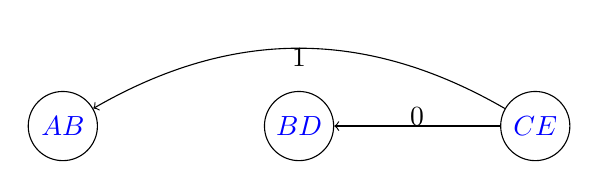
\begin{tikzpicture}[node distance = 3cm,auto,inner sep=0pt]
\node[state,text=blue,draw=black] (A) {$AB$};
\node[state,text=blue,draw=black] (B) [right of = A]  {$BD$};
\node[state,text=blue,draw=black] (C) [right of = B] {$CE$};
\path (B) edge [<-] node {$0$} (C);

\path (C) edge [->,bend right] node {$1$} (A);
\end{tikzpicture}
\end{center}

\hspace*{0.1cm} The testing graph for information losslessness is loop-free. The order of losslessness is $\mu = 1 + 2 = 3$. The length of the longest path of the graph is $1$.

\newpage
\begin{flushleft}
    \textbf{206}\hspace*{0.1cm} \textbf{$|$} \hspace*{0.1cm} {\small \texttt{Introduction to Automata Theory, Formal Languages and Computation}}
  \end{flushleft}
\vspace*{0.5cm}

$17.$ Test whether the following machine is information lossless or not. If lossless, find its order.

\vspace*{0.1cm}
\begin{center}
\begin{tabular}{ccc}
 \hline

 \hline

 \hline

 \hline
 & \multicolumn{2}{c}{Next State,O/P}\\
 \cline{2-3}
Present State & X=0           &   X=1\\
\hline
    A    &  B,1  & C,1 \\
    B    &  D,0  & E,0 \\
    C    &  A,1  & F,1 \\
    D    &  C,0  & B,0 \\
    E    &  F,1  & A,0 \\
    F    &  E,0  & D,0 \\
 \hline

 \hline

 \hline

 \hline
\end{tabular}
\end{center}

\large{\textbf{Solution:}} \small{First, we have to construct a testing table for information losslessness for testing whether the machine is information lossless or not. The testing table is divided into two halves.}

\large{\textbf{Solution:}} First, we have to construct a testing table for information losslessness for testing whether the machine is information lossless or not. The testing table is divided into two halves.

\begin{center}
  \begin{tabular}{ccc}
\hline

\hline

\hline

\hline
 & \multicolumn{2}{c}{Next State}\\
 \cline{2-3}
Present State & z = 0 & z = 1\\
\hline
 A &     --    &     BC     \\
 B &     DE    &     --     \\
 C &     --    &     AF     \\
 D &     BC    &     --     \\
 E &     --    &     AF     \\
 F &     DE    &     --     \\
\hline
 AF &    --      &     --  \\
 BC &    --      &     --  \\
 DE &    --      &     --  \\
\hline

\hline

\hline

\hline

  \end{tabular}
\end{center}

\hspace*{0.1cm} The testing table does not contain any repeated entry. The machine is an information lossless machine.\\
\hspace*{0.1cm} The testing graph for the machine is

\begin{center}
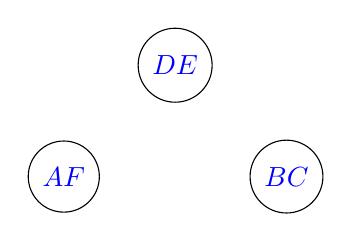
\begin{tikzpicture}[node distance = 2cm]
\node[state,text = blue] (A) {$DE$};
\node[state,text = blue] (B) [below left of = A] {$AF$};
\node[state,text = blue] (C) [below right of = A] {$BC$};

\end{tikzpicture}
\end{center}


\hspace*{0.1cm} The testing graph for information losslessness is loop-free. The order of losslessness is $\mu = 0 + 2 = 2$. The length of the longest path of the graph is 0.


\newpage

\begin{flushright}
\texttt{Finite State Machine} \hspace*{0.1cm}\textbf{$|$} \hspace*{0.1cm} \textbf{207}\hspace*{0.1cm}
\end{flushright}
\vspace*{0.5cm}


$18.$ Test whether the following machine is information lossless or not. If lossless, find its order.

\begin{center}
\begin{tabular}{ccc}
 \hline

 \hline

 \hline

 \hline
 & \multicolumn{2}{c}{Next State,O/P}\\
 \cline{2-3}
Present State & X=0           &   X=1\\
\hline
    A    &  B,0  & E,0 \\
    B    &  E,0  & D,0 \\
    C    &  D,1  & A,1 \\
    D    &  C,1  & E,0 \\
    E    &  B,0  & D,0 \\
 \hline

 \hline

 \hline

 \hline
\end{tabular}
\end{center}

\large{\textbf{Solution:}} First, we have to construct a testing table for information losslessness for testing whether the machine is information lossless or not. The testing table is divided into two halves.


\begin{center}
  \begin{tabular}{ccc}
\hline

\hline

\hline

\hline
 & \multicolumn{2}{c}{Next State}\\
 \cline{2-3}
Present State & z = 0 & z = 1\\
\hline
 A   &  BE  &   –- \\
 B   &  DE  &   –- \\
 C   &  A   &   D  \\
 D   &  E   &   C  \\
 E   &  BD  &   –- \\
\hline
 BD  &  (DE)(EE)  &   -–    \\
 BE  &  (BD)(DE)  &   –-    \\
 DE  &  (BE)(DE)  &   –-    \\
\hline

\hline

\hline

\hline

  \end{tabular}
\end{center}

The testing table contains repeated entry (EE). Therefore, the machine is a lossy machine.

$19.$ Test whether the following machine is information lossless or not. If lossless, find its order.

\begin{center}
  \begin{tabular}{ccc}
\hline

\hline

\hline

\hline
 & \multicolumn{2}{c}{Next State,O/P}\\
 \cline{2-3}
Present State & X = 0 & X = 1\\
\hline
  A    &    B, 1     &    C, 0 \\
  B    &    B, 1     &    D, 1 \\
  C    &    E, 1     &    B, 0 \\
  D    &    A, 0     &    E, 0 \\
  E    &    F, 0     &    D, 1 \\
  F    &    A, 1     &    D, 0 \\
\hline

\hline

\hline

\hline

  \end{tabular}
\end{center}

\large{\textbf{Solution:}} \small{First, we have to construct a testing table for information losslessness for testing whether the machine is information lossless or not. The testing table is divided into two halves.}

\newpage
\begin{flushleft}
    \textbf{208}\hspace*{0.1cm} \textbf{$|$} \hspace*{0.1cm} {\small \texttt{Introduction to Automata Theory, Formal Languages and Computation}}
  \end{flushleft}
\vspace*{0.5cm}


\begin{center}
  \begin{tabular}{ccc}
\hline

\hline

\hline

\hline
 & \multicolumn{2}{c}{Next State}\\
 \cline{2-3}
Present State & z = 0 & z = 1\\
\hline
 A    &   C    &       B     \\
 B    &   -–   &      (BD)   \\
 C    &   B    &       E     \\
 D    &  (AE)  &       -–    \\
 E    &   F    &       D     \\
 F    &   D    &       A     \\
\hline
 AE   &   CF   &       BD     \\
 BD   &   -–   &       -–     \\
 CF   &   BD   &       AE     \\
\hline

\hline

\hline

\hline

  \end{tabular}
\end{center}

\hspace*{0.1cm} The testing table does not contain any repeated entry. The machine is an information lossless machine.\\

\hspace*{0.1cm} The testing graph for the machine is

\begin{center}
\begin{tikzpicture}[node distance = 3cm,auto]
\node[state,text = blue] (A) {$CF$};
\path (A) edge [->] node {$1$} (B);
\path (B) edge [->] node {$0$} (A);
\path (A) edge [->] node {$0$} (C);
\path (B) edge [->] node {$1$} (C);
\node[state,text = blue] (B) [below left of = A] {$AE$};
\node[state,text = blue] (C) [below right of = A] {$BD$};

\end{tikzpicture}
\end{center}

\hspace*{0.1cm} The testing graph contains a loop. So, the machine is not information lossless of finite order. The order of losslessness $\mu = 2 + 2 = 4$. The length of the longest path of the graph is 2. 

$20.$ The state table of a finite state machine M is as follows. Check whether the machine M is information lossless. If it is information lossless, then determine the order of losslessness.\\

\begin{flushright}
  [WBUT 2003]
\end{flushright}
\vspace*{0.1cm}


\begin{center}
  \begin{tabular}{ccc}
\hline

\hline

\hline

\hline
 & \multicolumn{2}{c}{Next State,O/P}\\
 \cline{2-3}
Present State & X = 0 & X = 1\\
\hline
 A    &   A, 0   &   B, 0  \\
 B    &   C, 0   &   D, 0  \\
 C    &   D, 1   &   C, 1  \\
 D    &   B, 1   &   A, 0  \\
\hline

\hline

\hline

\hline

  \end{tabular}
\end{center}
\vspace*{0.1cm}


\large{\textbf{Solution:}} \small{First, we have to construct a testing table for information losslessness for testing whether the machine is information lossless or not. The testing table is}

\end{document} 